\documentclass[a4paper,10pt]{article} % {{{
\usepackage{listings,amssymb,amsmath,amsthm,graphicx,float,hyperref}

\hypersetup{
    colorlinks=false,
    pdfborder={0 0 0},
}
\newcommand{\tsup}[1]{\ensuremath{\sp{\text{#1}}}}

% Template coming from Pygments (pygmentize with "-O full,preamble")

\usepackage{fancyvrb}
\usepackage{color}

\makeatletter
\def\PY@reset{\let\PY@it=\relax \let\PY@bf=\relax%
    \let\PY@ul=\relax \let\PY@tc=\relax%
    \let\PY@bc=\relax \let\PY@ff=\relax}
\def\PY@tok#1{\csname PY@tok@#1\endcsname}
\def\PY@toks#1+{\ifx\relax#1\empty\else%
    \PY@tok{#1}\expandafter\PY@toks\fi}
\def\PY@do#1{\PY@bc{\PY@tc{\PY@ul{%
    \PY@it{\PY@bf{\PY@ff{#1}}}}}}}
\def\PY#1#2{\PY@reset\PY@toks#1+\relax+\PY@do{#2}}

\def\PY@tok@gd{\def\PY@tc##1{\textcolor[rgb]{0.63,0.00,0.00}{##1}}}
\def\PY@tok@gu{\let\PY@bf=\textbf\def\PY@tc##1{\textcolor[rgb]{0.50,0.00,0.50}{##1}}}
\def\PY@tok@gt{\def\PY@tc##1{\textcolor[rgb]{0.00,0.25,0.82}{##1}}}
\def\PY@tok@gs{\let\PY@bf=\textbf}
\def\PY@tok@gr{\def\PY@tc##1{\textcolor[rgb]{1.00,0.00,0.00}{##1}}}
\def\PY@tok@cm{\def\PY@tc##1{\textcolor[rgb]{0.50,0.50,0.50}{##1}}}
\def\PY@tok@vg{\let\PY@bf=\textbf\def\PY@tc##1{\textcolor[rgb]{0.82,0.44,0.00}{##1}}}
\def\PY@tok@m{\let\PY@bf=\textbf\def\PY@tc##1{\textcolor[rgb]{0.38,0.00,0.88}{##1}}}
\def\PY@tok@mh{\let\PY@bf=\textbf\def\PY@tc##1{\textcolor[rgb]{0.00,0.31,0.50}{##1}}}
\def\PY@tok@cs{\let\PY@bf=\textbf\def\PY@tc##1{\textcolor[rgb]{0.80,0.00,0.00}{##1}}}
\def\PY@tok@ge{\let\PY@it=\textit}
\def\PY@tok@vc{\def\PY@tc##1{\textcolor[rgb]{0.19,0.38,0.56}{##1}}}
\def\PY@tok@il{\let\PY@bf=\textbf\def\PY@tc##1{\textcolor[rgb]{0.00,0.00,0.82}{##1}}}
\def\PY@tok@go{\def\PY@tc##1{\textcolor[rgb]{0.50,0.50,0.50}{##1}}}
\def\PY@tok@cp{\def\PY@tc##1{\textcolor[rgb]{0.31,0.44,0.56}{##1}}}
\def\PY@tok@gi{\def\PY@tc##1{\textcolor[rgb]{0.00,0.63,0.00}{##1}}}
\def\PY@tok@gh{\let\PY@bf=\textbf\def\PY@tc##1{\textcolor[rgb]{0.00,0.00,0.50}{##1}}}
\def\PY@tok@ni{\let\PY@bf=\textbf\def\PY@tc##1{\textcolor[rgb]{0.50,0.00,0.00}{##1}}}
\def\PY@tok@nl{\let\PY@bf=\textbf\def\PY@tc##1{\textcolor[rgb]{0.56,0.44,0.00}{##1}}}
\def\PY@tok@nn{\let\PY@bf=\textbf\def\PY@tc##1{\textcolor[rgb]{0.05,0.52,0.71}{##1}}}
\def\PY@tok@no{\let\PY@bf=\textbf\def\PY@tc##1{\textcolor[rgb]{0.00,0.19,0.38}{##1}}}
\def\PY@tok@na{\def\PY@tc##1{\textcolor[rgb]{0.00,0.00,0.75}{##1}}}
\def\PY@tok@nb{\def\PY@tc##1{\textcolor[rgb]{0.00,0.44,0.13}{##1}}}
\def\PY@tok@nc{\let\PY@bf=\textbf\def\PY@tc##1{\textcolor[rgb]{0.69,0.00,0.38}{##1}}}
\def\PY@tok@nd{\let\PY@bf=\textbf\def\PY@tc##1{\textcolor[rgb]{0.31,0.31,0.31}{##1}}}
\def\PY@tok@ne{\let\PY@bf=\textbf\def\PY@tc##1{\textcolor[rgb]{0.94,0.00,0.00}{##1}}}
\def\PY@tok@nf{\let\PY@bf=\textbf\def\PY@tc##1{\textcolor[rgb]{0.00,0.38,0.69}{##1}}}
\def\PY@tok@si{\def\PY@bc##1{\colorbox[rgb]{0.88,0.88,0.88}{##1}}}
\def\PY@tok@s2{\def\PY@bc##1{\colorbox[rgb]{1.00,0.94,0.94}{##1}}}
\def\PY@tok@vi{\def\PY@tc##1{\textcolor[rgb]{0.19,0.19,0.69}{##1}}}
\def\PY@tok@nt{\def\PY@tc##1{\textcolor[rgb]{0.00,0.44,0.00}{##1}}}
\def\PY@tok@nv{\def\PY@tc##1{\textcolor[rgb]{0.56,0.38,0.19}{##1}}}
\def\PY@tok@s1{\def\PY@bc##1{\colorbox[rgb]{1.00,0.94,0.94}{##1}}}
\def\PY@tok@gp{\let\PY@bf=\textbf\def\PY@tc##1{\textcolor[rgb]{0.78,0.36,0.04}{##1}}}
\def\PY@tok@sh{\def\PY@bc##1{\colorbox[rgb]{1.00,0.94,0.94}{##1}}}
\def\PY@tok@ow{\let\PY@bf=\textbf\def\PY@tc##1{\textcolor[rgb]{0.00,0.00,0.00}{##1}}}
\def\PY@tok@sx{\def\PY@tc##1{\textcolor[rgb]{0.82,0.13,0.00}{##1}}
    \def\PY@bc##1{\colorbox[rgb]{1.00,0.94,0.94}{##1}}}
\def\PY@tok@bp{\def\PY@tc##1{\textcolor[rgb]{0.00,0.44,0.13}{##1}}}
\def\PY@tok@c1{\def\PY@tc##1{\textcolor[rgb]{0.50,0.50,0.50}{##1}}}
\def\PY@tok@kc{\let\PY@bf=\textbf\def\PY@tc##1{\textcolor[rgb]{0.00,0.50,0.00}{##1}}}
\def\PY@tok@c{\def\PY@tc##1{\textcolor[rgb]{0.50,0.50,0.50}{##1}}}
\def\PY@tok@mf{\let\PY@bf=\textbf\def\PY@tc##1{\textcolor[rgb]{0.38,0.00,0.88}{##1}}}
\def\PY@tok@err{\def\PY@tc##1{\textcolor[rgb]{0.94,0.00,0.00}{##1}}
    \def\PY@bc##1{\colorbox[rgb]{0.94,0.63,0.63}{##1}}}
\def\PY@tok@kd{\let\PY@bf=\textbf\def\PY@tc##1{\textcolor[rgb]{0.00,0.50,0.00}{##1}}}
\def\PY@tok@ss{\def\PY@tc##1{\textcolor[rgb]{0.63,0.38,0.00}{##1}}}
\def\PY@tok@sr{\def\PY@tc##1{\textcolor[rgb]{0.00,0.00,0.00}{##1}}
    \def\PY@bc##1{\colorbox[rgb]{1.00,0.94,1.00}{##1}}}
\def\PY@tok@mo{\let\PY@bf=\textbf\def\PY@tc##1{\textcolor[rgb]{0.25,0.00,0.88}{##1}}}
\def\PY@tok@mi{\let\PY@bf=\textbf\def\PY@tc##1{\textcolor[rgb]{0.00,0.00,0.82}{##1}}}
\def\PY@tok@kn{\let\PY@bf=\textbf\def\PY@tc##1{\textcolor[rgb]{0.00,0.50,0.00}{##1}}}
\def\PY@tok@o{\def\PY@tc##1{\textcolor[rgb]{0.19,0.19,0.19}{##1}}}
\def\PY@tok@kr{\let\PY@bf=\textbf\def\PY@tc##1{\textcolor[rgb]{0.00,0.50,0.00}{##1}}}
\def\PY@tok@s{\def\PY@bc##1{\colorbox[rgb]{1.00,0.94,0.94}{##1}}}
\def\PY@tok@kp{\let\PY@bf=\textbf\def\PY@tc##1{\textcolor[rgb]{0.00,0.19,0.50}{##1}}}
\def\PY@tok@w{\def\PY@tc##1{\textcolor[rgb]{0.73,0.73,0.73}{##1}}}
\def\PY@tok@kt{\let\PY@bf=\textbf\def\PY@tc##1{\textcolor[rgb]{0.19,0.19,0.56}{##1}}}
\def\PY@tok@sc{\def\PY@tc##1{\textcolor[rgb]{0.00,0.25,0.82}{##1}}}
\def\PY@tok@sb{\def\PY@bc##1{\colorbox[rgb]{1.00,0.94,0.94}{##1}}}
\def\PY@tok@k{\let\PY@bf=\textbf\def\PY@tc##1{\textcolor[rgb]{0.00,0.50,0.00}{##1}}}
\def\PY@tok@se{\let\PY@bf=\textbf\def\PY@tc##1{\textcolor[rgb]{0.38,0.38,0.38}{##1}}
   } % \def\PY@bc##1{\colorbox[rgb]{1.00,0.94,0.94}{##1}}}
\def\PY@tok@sd{\def\PY@tc##1{\textcolor[rgb]{0.82,0.25,0.13}{##1}}}

\def\PYZbs{\char`\\}
\def\PYZus{\char`\_}
\def\PYZob{\char`\{}
\def\PYZcb{\char`\}}
\def\PYZca{\char`\^}
% for compatibility with earlier versions
\def\PYZat{@}
\def\PYZlb{[}
\def\PYZrb{]}
\makeatother



% gebruik '\and' tussen authors, '\\' voor extra info over een author.
\author{Harm Dermois (5027963) \and Joris Stork (6185320) \and
Lucas Swartsenburg (6174388) \and Sander van Veen (6167969)}

\title{Cobots and Sun SPOTs: a robotics project}

% }}}

\begin{document}

\maketitle

\abstract{}

\pagebreak

\tableofcontents

\pagebreak

\section{Introduction} % {{{

This project concludes our team's involvement in a January 2011 robotics course
at the University of Amsterdam. The team consists of four second-year UvA
students enrolled for the BSc in Computer Science. The overall aim of this
project has been to address the challenges inherent in programming a microcontroller
based mobile robot and handling communication between multiple, differing
devices as might be required for many robotics applications.

In this project, our team was given the task, firstly, of ``resuscitating'' the
UvA's Java-programmable ``Jobot'' robots, whose software development platform
had become defunct and inoperative. Our second task was to combine the Jobots'
mobility and sensing capabilities with the enhanced communications, sensing and
processing functionality of Sun SPOTs -- wireless sensor network devices from
the Sun Labs stable. In this way, we hoped to achieve a few things, namely to:

\begin{itemize}
    \item write, compile and load programs from scratch for a PIC based
    microcontroller board;
    \item create drivers for the servos and sensors connected to the board
    mentioned above;
    \item further explore the Sun SPOTs' sensing and communications
    characteristics through those devices' Java frameworks;
    \item build a data communication channel between the Sun SPOTs and the
    standard microcontrollers on the Jobots. Investigate whether this could be
    achieved over an $I^2C$ bus;
    \item design an interface between our respective software implementations on
    the Jobot and on the Sun SPOTs;
    \item build a remote control system using the above interface;
    \item attempt some basic robot activities using our adapted, Sun SPOT
    controlled robot(s), such as: obstacle avoidance; reaching a goal;
    recognising a fellow robot; following a fellow robot, and so on, and;
    \item learn to work with embedded chips and low-level signal handling.
\end{itemize}

Strict time and resource limitations took precedence over any adherence
to pre-formulated goals and methods. That said, our project was successful,
and our team achieved a bonus on the way.

This report describes the principal materials at our disposal and our approach
to completing the given project tasks. Our methods are described per challenge,
in chronological order of their occurrence, for each of the Sun SPOT; Cobot; and
Sun SPOT -- Cobot combination. This approach reflects the exploratory nature of
the project, in which a string of unexpected obstacles dictated the structure of
our efforts over the past two weeks.

% }}}

%\section{Materials} % {{{
%
%Appendix
%
%% TODO: Is it wise to store this section in the appendix or here?
%
%% }}}

\pagebreak

\section{Methods} % {{{

This section provides an overview of the materials used in this project. More
detailed specifications of materials used in this project are listed in appendix
\ref{app:robot-hardware}, as relevant.

\subsection{Hardware} % {{{

Two hardware devices formed the centrepiece of this project:

\begin{itemize}
    \item a set of three ``Jobots'', re-christened by our group to
    ``Cobots'': three-wheeled, battery powered and PIC microcontroller-based mobile
    robots, about 10cm high and 25cm across, built around a rigid aluminium frame;
    and
    \item a set of three Sun SPOTs: battery powered wireless sensor network
    devices ranging in number from three to six, and each a little bigger than a
    matchbox.
\end{itemize}

\noindent Other hardware included:

\begin{itemize}
    \item a portable digital oscilloscope, for measuring voltages on the various
    I/O pins on the SUN SPOTs and microcontroller boards (as well as the odd
    misbehaving battery);
    \item a USB compatible Microchip programming device designed to load compiled code
    onto the 8 bit PIC microcontroller;
    \item an 8P8C type connector attached on the port location marked ``J1'' on
    one of the Cobot' microcontroller boards;
    \item a USB to RS-232 adapter cable;
    \item standard soldering equipment;
    \item pins and wires adapted for the Sun SPOTs' as well as the Cobots' I/O
    connectors; and
    \item two potential dividers built by our university department for the
    purpose of converting a 5V input voltage from the Cobot's microcontroller
    board to the 3V output voltage specified for the Sun SPOTs;
\end{itemize}

% }}}

\subsection{Establishing COM-to-USB connection} % {{{
\label{sub:Establishing COM-to-USB connection}

In order to see if a Cobot or Hemisson is performing some action, it is wise to
write debug information to a file or serial port. In this case, the serial port
is available on both robots, which will provide us a ``real-time'' view of the
robot's current and next actions to perform. Sander developed the following code
to be able to command the Hemisson robot using a python console connected with a
serial port:

\begin{Verbatim}[commandchars=\\\{\}]
\PY{c}{#!/usr/bin/env python}
\PY{c}{#}
\PY{c}{# This script is used to read and write data from/to the COM-to-USB port.}
\PY{c}{# Created by Sander van Veen <sandervv@gmail.com>, Jan 27, 2011.}
\PY{c}{# This script is public domain; feel free to do anything with it you want.}
\PY{c}{#}
\PY{c}{# Example invocation: $ python -i hemisson.py}

\PY{k+kn}{from} \PY{n+nn}{serial} \PY{k+kn}{import} \PY{n}{Serial}\PY{p}{,} \PY{n}{PARITY\PYZus{}NONE}\PY{p}{,} \PY{n}{EIGHTBITS}\PY{p}{,} \PY{n}{STOPBITS\PYZus{}ONE}
\PY{k+kn}{from} \PY{n+nn}{time} \PY{k+kn}{import} \PY{n}{sleep}

\PY{k}{class} \PY{n+nc}{HemissonException}\PY{p}{(}\PY{n+ne}{Exception}\PY{p}{)}\PY{p}{:}
    \PY{k}{def} \PY{n+nf}{\PYZus{}\PYZus{}init\PYZus{}\PYZus{}}\PY{p}{(}\PY{n+nb+bp}{self}\PY{p}{,} \PY{n}{value}\PY{p}{)}\PY{p}{:}
        \PY{n+nb+bp}{self}\PY{o}{.}\PY{n}{value} \PY{o}{=} \PY{n}{value}

    \PY{k}{def} \PY{n+nf}{\PYZus{}\PYZus{}str\PYZus{}\PYZus{}}\PY{p}{(}\PY{n+nb+bp}{self}\PY{p}{)}\PY{p}{:}
        \PY{k}{return} \PY{n+nb}{repr}\PY{p}{(}\PY{n+nb+bp}{self}\PY{o}{.}\PY{n}{value}\PY{p}{)}

\PY{k}{class} \PY{n+nc}{Hemisson}\PY{p}{:}
    \PY{k}{def} \PY{n+nf}{\PYZus{}\PYZus{}init\PYZus{}\PYZus{}}\PY{p}{(}\PY{n+nb+bp}{self}\PY{p}{)}\PY{p}{:}
        \PY{l+s+sd}{"""}
        \PY{l+s+sd}{Initialise the serial connection to the Hemisson robot.}
        \PY{l+s+sd}{"""}

        \PY{c}{# Initialise serial connection on /dev/ttyUSB0}
        \PY{n+nb+bp}{self}\PY{o}{.}\PY{n}{serial} \PY{o}{=} \PY{n}{Serial}\PY{p}{(}\PY{l+m+mi}{0}\PY{p}{)}
        \PY{n+nb+bp}{self}\PY{o}{.}\PY{n}{serial}\PY{o}{.}\PY{n}{setParity}\PY{p}{(}\PY{n}{PARITY\PYZus{}NONE}\PY{p}{)}
        \PY{n+nb+bp}{self}\PY{o}{.}\PY{n}{serial}\PY{o}{.}\PY{n}{setByteSize}\PY{p}{(}\PY{n}{EIGHTBITS}\PY{p}{)}
        \PY{n+nb+bp}{self}\PY{o}{.}\PY{n}{serial}\PY{o}{.}\PY{n}{setStopbits}\PY{p}{(}\PY{n}{STOPBITS\PYZus{}ONE}\PY{p}{)}
        \PY{n+nb+bp}{self}\PY{o}{.}\PY{n}{serial}\PY{o}{.}\PY{n}{setBaudrate}\PY{p}{(}\PY{l+m+mi}{115200}\PY{p}{)}

        \PY{c}{# Connection established, read welcome message from Hemisson.}
        \PY{k}{print} \PY{l+s}{'}\PY{l+s}{i Initialised serial connection }\PY{l+s}{"}\PY{l+s+si} \PY{n+nb+bp}{self}\PY{o}{.}\PY{n}{serial}\PY{o}{.}\PY{n}{portstr}
        \PY{n+nb+bp}{self}\PY{o}{.}\PY{n}{serial}\PY{o}{.}\PY{n}{write}\PY{p}{(}\PY{n+nb}{chr}\PY{p}{(}\PY{l+m+mi}{254}\PY{p}{)}\PY{o}{+}\PY{l+s}{'}\PY{l+s+se}{\PYZbs{}r}\PY{l+s}{'}\PY{p}{)}
        \PY{n+nb+bp}{self}\PY{o}{.}\PY{n}{readline}\PY{p}{(}\PY{p}{)}
        \PY{n+nb+bp}{self}\PY{o}{.}\PY{n}{readline}\PY{p}{(}\PY{p}{)}
        \PY{n+nb+bp}{self}\PY{o}{.}\PY{n}{readline}\PY{p}{(}\PY{p}{)}

    \PY{k}{def} \PY{n+nf}{\PYZus{}\PYZus{}delete\PYZus{}\PYZus{}}\PY{p}{(}\PY{n+nb+bp}{self}\PY{p}{)}\PY{p}{:}
        \PY{l+s+sd}{"""}
        \PY{l+s+sd}{Disconnect the serial connnection to the Hemisson robot.}
        \PY{l+s+sd}{"""}

        \PY{k}{print} \PY{l+s}{'}\PY{l+s}{i Destroying serial connection }\PY{l+s}{"}\PY{l+s+si} \PY{n+nb+bp}{self}\PY{o}{.}\PY{n}{serial}\PY{o}{.}\PY{n}{portstr}
        \PY{n+nb+bp}{self}\PY{o}{.}\PY{n}{write}\PY{p}{(}\PY{n+nb}{chr}\PY{p}{(}\PY{l+m+mi}{8}\PY{p}{)}\PY{p}{)}
        \PY{n+nb+bp}{self}\PY{o}{.}\PY{n}{serial}\PY{o}{.}\PY{n}{close}\PY{p}{(}\PY{p}{)}

    \PY{k}{def} \PY{n+nf}{beep}\PY{p}{(}\PY{n+nb+bp}{self}\PY{p}{,} \PY{n}{state}\PY{p}{)}\PY{p}{:}
        \PY{l+s+sd}{"""}
        \PY{l+s+sd}{Generates a continuous beep, depending on state (0 = Off, 1 = On).}
        \PY{l+s+sd}{"""}

        \PY{k}{if} \PY{n}{state} \PY{o+ow}{not} \PY{o+ow}{in} \PY{p}{(}\PY{l+m+mi}{0}\PY{p}{,} \PY{l+m+mi}{1}\PY{p}{)}\PY{p}{:}
            \PY{k}{raise} \PY{n}{HemissionException}\PY{p}{(}\PY{l+s}{'}\PY{l+s}{Beep state should be 0 (Off) or 1 (On).}\PY{l+s}{'}\PY{p}{)}

        \PY{n+nb+bp}{self}\PY{o}{.}\PY{n}{write}\PY{p}{(}\PY{l+s}{'}\PY{l+s}{H,}\PY{l+s+si} \PY{n}{state}\PY{p}{)}
        \PY{n+nb+bp}{self}\PY{o}{.}\PY{n}{readline}\PY{p}{(}\PY{p}{)}

    \PY{k}{def} \PY{n+nf}{drive}\PY{p}{(}\PY{n+nb+bp}{self}\PY{p}{)}\PY{p}{:}
        \PY{l+s+sd}{"""}
        \PY{l+s+sd}{Drive forward (setting both wheel's drive speed to '2').}
        \PY{l+s+sd}{"""}

        \PY{n+nb+bp}{self}\PY{o}{.}\PY{n}{set\PYZus{}speed}\PY{p}{(}\PY{l+m+mi}{2}\PY{p}{)}

    \PY{k}{def} \PY{n+nf}{get\PYZus{}switches}\PY{p}{(}\PY{n+nb+bp}{self}\PY{p}{)}\PY{p}{:}
        \PY{l+s+sd}{"""}
        \PY{l+s+sd}{Read the current status of the four top switches. Possible values are 0}
        \PY{l+s+sd}{(= robot's right handside) and 1 (= robot's left handside). The first}
        \PY{l+s+sd}{value is the value of the first switch from the front of the robot.}
        \PY{l+s+sd}{"""}

        \PY{n+nb+bp}{self}\PY{o}{.}\PY{n}{write}\PY{p}{(}\PY{l+s}{'}\PY{l+s}{I}\PY{l+s}{'}\PY{p}{)}
        \PY{n+nb+bp}{self}\PY{o}{.}\PY{n}{readline}\PY{p}{(}\PY{p}{)}

    \PY{k}{def} \PY{n+nf}{set\PYZus{}speed}\PY{p}{(}\PY{n+nb+bp}{self}\PY{p}{,} \PY{n}{left}\PY{p}{,} \PY{n}{right}\PY{o}{=}\PY{n+nb+bp}{None}\PY{p}{)}\PY{p}{:}
        \PY{l+s+sd}{"""}
        \PY{l+s+sd}{Set driving speed of left and right wheel. If only the left wheel drive}
        \PY{l+s+sd}{speed is given, the right wheel's drive speed is set to the left}
        \PY{l+s+sd}{wheel's drive speed.}
        \PY{l+s+sd}{"""}

        \PY{k}{if} \PY{n}{right} \PY{o}{==} \PY{n+nb+bp}{None}\PY{p}{:}
            \PY{n}{right} \PY{o}{=} \PY{n}{left}

        \PY{k}{if} \PY{o+ow}{not}\PY{p}{(} \PY{o}{-}\PY{l+m+mi}{9} \PY{o}{<}\PY{o}{=} \PY{n}{left} \PY{o}{<}\PY{o}{=} \PY{l+m+mi}{9} \PY{o+ow}{and} \PY{o}{-}\PY{l+m+mi}{9} \PY{o}{<}\PY{o}{=} \PY{n}{right} \PY{o}{<}\PY{o}{=} \PY{l+m+mi}{9}\PY{p}{)}\PY{p}{:}
            \PY{k}{raise} \PY{n}{HemissonException}\PY{p}{(}
                \PY{l+s}{'}\PY{l+s}{Keep the wheel drive speed value between -9 and 9.}\PY{l+s}{'}\PY{p}{)}

        \PY{n+nb+bp}{self}\PY{o}{.}\PY{n}{write}\PY{p}{(}\PY{l+s}{'}\PY{l+s}{D,}\PY{l+s+si}{%d}\PY{l+s}{,}\PY{l+s+si} \PY{p}{(}\PY{n}{left}\PY{p}{,} \PY{n}{right}\PY{p}{)}\PY{p}{)}
        \PY{n+nb+bp}{self}\PY{o}{.}\PY{n}{readline}\PY{p}{(}\PY{p}{)}

    \PY{k}{def} \PY{n+nf}{stop}\PY{p}{(}\PY{n+nb+bp}{self}\PY{p}{)}\PY{p}{:}
        \PY{l+s+sd}{"""}
        \PY{l+s+sd}{Stop moving forward (setting both wheel's drive speed to zero).}
        \PY{l+s+sd}{"""}

        \PY{n+nb+bp}{self}\PY{o}{.}\PY{n}{write}\PY{p}{(}\PY{l+s}{'}\PY{l+s}{D,0,0}\PY{l+s}{'}\PY{p}{)}
        \PY{n+nb+bp}{self}\PY{o}{.}\PY{n}{readline}\PY{p}{(}\PY{p}{)}

    \PY{k}{def} \PY{n+nf}{readline}\PY{p}{(}\PY{n+nb+bp}{self}\PY{p}{)}\PY{p}{:}
        \PY{l+s+sd}{"""}
        \PY{l+s+sd}{Read a single newline terminated line from the serial connection.}
        \PY{l+s+sd}{"""}

        \PY{k}{print} \PY{l+s}{'}\PY{l+s}{< }\PY{l+s+si} \PY{n+nb+bp}{self}\PY{o}{.}\PY{n}{serial}\PY{o}{.}\PY{n}{readline}\PY{p}{(}\PY{p}{)}\PY{p}{[}\PY{p}{:}\PY{o}{-}\PY{l+m+mi}{1}\PY{p}{]}

    \PY{k}{def} \PY{n+nf}{remote\PYZus{}version}\PY{p}{(}\PY{n+nb+bp}{self}\PY{p}{)}\PY{p}{:}
        \PY{l+s+sd}{"""}
        \PY{l+s+sd}{Display version of the HemiOS running on the connected Hemisson robot.}
        \PY{l+s+sd}{"""}

        \PY{n+nb+bp}{self}\PY{o}{.}\PY{n}{write}\PY{p}{(}\PY{l+s}{'}\PY{l+s}{B}\PY{l+s}{'}\PY{p}{)}
        \PY{n+nb+bp}{self}\PY{o}{.}\PY{n}{readline}\PY{p}{(}\PY{p}{)}

    \PY{k}{def} \PY{n+nf}{reset}\PY{p}{(}\PY{n+nb+bp}{self}\PY{p}{)}\PY{p}{:}
        \PY{l+s+sd}{"""}
        \PY{l+s+sd}{Reset the robot's processor as if the On/Off switch is cycled.}
        \PY{l+s+sd}{"""}

        \PY{n+nb+bp}{self}\PY{o}{.}\PY{n}{serial}\PY{o}{.}\PY{n}{write}\PY{p}{(}\PY{l+s}{'}\PY{l+s}{Z}\PY{l+s}{'}\PY{p}{)}
        \PY{n+nb+bp}{self}\PY{o}{.}\PY{n}{readline}\PY{p}{(}\PY{p}{)}

    \PY{k}{def} \PY{n+nf}{write}\PY{p}{(}\PY{n+nb+bp}{self}\PY{p}{,} \PY{n}{msg}\PY{p}{)}\PY{p}{:}
        \PY{l+s+sd}{"""}
        \PY{l+s+sd}{Write a message through the serial connection to the Hemisson robot.}
        \PY{l+s+sd}{"""}

        \PY{k}{print} \PY{l+s}{'}\PY{l+s}{> }\PY{l+s+si} \PY{n}{msg}
        \PY{n+nb+bp}{self}\PY{o}{.}\PY{n}{serial}\PY{o}{.}\PY{n}{write}\PY{p}{(}\PY{n}{msg}\PY{o}{+}\PY{l+s}{'}\PY{l+s+se}{\PYZbs{}n}\PY{l+s+se}{\PYZbs{}r}\PY{l+s}{'}\PY{p}{)}

\PY{k}{if} \PY{n}{\PYZus{}\PYZus{}name\PYZus{}\PYZus{}} \PY{o}{==} \PY{l+s}{'}\PY{l+s}{\PYZus{}\PYZus{}main\PYZus{}\PYZus{}}\PY{l+s}{'}\PY{p}{:}
    \PY{n}{robot} \PY{o}{=} \PY{n}{Hemisson}\PY{p}{(}\PY{p}{)}
    \PY{n}{robot}\PY{o}{.}\PY{n}{remote\PYZus{}version}\PY{p}{(}\PY{p}{)}
    \PY{n}{robot}\PY{o}{.}\PY{n}{get\PYZus{}switches}\PY{p}{(}\PY{p}{)}

    \PY{k}{for} \PY{n}{i} \PY{o+ow}{in} \PY{n+nb}{range}\PY{p}{(}\PY{l+m+mi}{4}\PY{p}{)}\PY{p}{:}
        \PY{n}{robot}\PY{o}{.}\PY{n}{set\PYZus{}speed}\PY{p}{(}\PY{l+m+mi}{4}\PY{p}{)}
        \PY{n}{sleep}\PY{p}{(}\PY{l+m+mi}{2}\PY{p}{)}
        \PY{n}{robot}\PY{o}{.}\PY{n}{set\PYZus{}speed}\PY{p}{(}\PY{o}{-}\PY{l+m+mi}{4}\PY{p}{,}\PY{l+m+mi}{4}\PY{p}{)}
        \PY{n}{sleep}\PY{p}{(}\PY{l+m+mf}{1.5}\PY{p}{)}

    \PY{n}{robot}\PY{o}{.}\PY{n}{stop}\PY{p}{(}\PY{p}{)}
\end{Verbatim}


% }}}

\subsection{Cobot preparations} % {{{

To program the Cobot we built a toolchain consisting of the following mixture of
pre-existing and custom-made software tools:

\begin{itemize}
    \item source code and compiled code for the Cobot, stored in a common
    working directory on UvA's science department servers;
    \item  the above directory mounted on a windows virtual machine and a Linux
    laptop over SSHFS\footnote{Secure SHell File System};
    \item Microchip's proprietary compiler for the Cobot's PIC microcontroller,
    running on the Windows virtual machine;
    \item our own python script, \texttt{compile.py}, running on the windows
    virtual machine: this automatically compiles the Cobot source code on the
    remote server when it changes;
    \item a python script on the Linux laptop to send commands to and read program
    output from the Cobot over the Cobot's RS-232 serial port;
\end{itemize}

For the Sun SPOT we used the % TODO: Lucas' software setup.


% }}}

\subsection{Cobot} % {{{

% TODO: our initial approach

% TODO: write a general approach to solve the problems occurred during
% development of Cobot's code. -- what does this mean?

\subsubsection{Toolchain used to program the Cobot} % {{{
\label{ssub:Toolchain used to program the Cobot}

First, we connected the shared directory using SSHFS:
\begin{verbatim}
$ sshfs USERNAME@deze.science.uva.nl:~/ ~/sremote -C -o cache=no
\end{verbatim}

The argument \texttt{-C} enables data compression during the transfer and
\texttt{-o cache=no} disables the file system cache (e.g. stat will respond with
the most recent data). If we did not disable the file system cache, the overall
duration of the toolchain is larger due to the default four seconds file system
cache. These four seconds are visible when the Mac machine running the Windows
VM was waiting for the source file to update and the second time when the Linux
machine was waiting for the hex file to update. Disabling the file system cache
reduced the overall toolchain process by four to eight seconds. Data compression
did not reduce the overall process that much, but we used it because we were
transferring text files (and those benefit for compression mostly).

Once we had the shared directory mounted on both the Linux and Mac machine, we
could transfer data between the Windows virtual machine and the Linux machine.
\footnote{Windows does not support SSHFS easily, and because we weren't working
actively a Windows machine, we started a virtual machine on the Mac.} The
Windows virtual machine started the compilation daemon (using \texttt{\$ python
compile.py}) and the Linux machine started the programming daemon (using
\texttt{python upload.py}).\footnote{See appendix for the source code of these
daemons.} Both daemons use the modification time of the source respectively the
compiled hex file to determine if the daemon should perform an action.

The programmer daemon uses the ``piklab'' package (in Debian-based
distributions: \texttt{sudo apt-get install piklab}) to write the hex file to
the Jobot. Be aware of the fact that piklab does not program the Jobot's
microcontroller right away, it is necessary to use the ICD2 Programmer, since
it is not possible to program the Jobot directly. The daemon will spawn a
sub process executing the Makefile's default target. The default target will
execute the following commands to program the Jobot:

\begin{verbatim}
$ sudo piklab-prog --port usb -p icd2 -d 18F450 -c connect
$ sudo piklab-prog --port usb -p icd2 -d 18F450 -c program file.hex
\end{verbatim}

It was necessary the execute these commands using \texttt{sudo}, because
piklab was not able to lock the USB-to-COM port otherwise. The second command
will also verify the programming process, thus verifying if the Jobot's
microcontroller contains the hex file we were uploading.

% }}}

\subsubsection{Controlling the actuators} % {{{
\label{sub:Cobot implementation}

Since there was no manual or documentation available about the toolchain, nor
about the internals of the Jobot, the first week's progress of this assignment
was slow. Most of the time, we were trying to solve problems and looking for
more information about the microcontroller and servos on the internet.
Eventually, when all tools for the toolchain were obtained and successfully
working together, we were able to run example code on the Jobot. This was the
breakthrough we were waiting for: we were able to write our own code and program
the Jobot with our compiled source code.

When we were using the PCH version of the CCS C compiler, we found some example
source code in the directory of the CCS C compiler. We modified the example code
to proof the microcontroller can do something, and programmed this modified code
on the Jobot's microcontroller:

\begin{Verbatim}[commandchars=\\\{\}]
\PY{c+c1}{// Device configuration: 20 Mhz processor and enable rs232,}
\PY{c+c1}{// which is the COM port. The COM port uses a baudrate of 9600.}
\PY{c+cp}{#}\PY{c+cp}{if defined(\PYZus{}\PYZus{}PCH\PYZus{}\PYZus{})}
\PY{c+cp}{#}\PY{c+cp}{include "18f452.h"}
\PY{c+cp}{#}\PY{c+cp}{fuses HS,NOPROTECT}
\PY{c+cp}{#}\PY{c+cp}{use delay(clock=20000000)}
\PY{c+cp}{#}\PY{c+cp}{use rs232(baud=9600, xmit=PIN\PYZus{}C6, rcv=PIN\PYZus{}C7)}
\PY{c+cp}{#}\PY{c+cp}{endif}

\PY{k+kt}{void} \PY{n+nf}{main}\PY{p}{(}\PY{p}{)} \PY{p}{\PYZob{}}
    \PY{c+c1}{// Set B pins to 'output' mode}
    \PY{n}{set\PYZus{}tris\PYZus{}b}\PY{p}{(}\PY{l+m+mi}{0}\PY{p}{)}\PY{p}{;}

    \PY{c+c1}{// Blink two LEDs (located on the microcontroller board).}
    \PY{c+c1}{// Wait for 2 ms between toggling the pins' value.}
    \PY{k}{while}\PY{p}{(}\PY{l+m+mi}{1}\PY{p}{)} \PY{p}{\PYZob{}}
        \PY{n}{output\PYZus{}high}\PY{p}{(}\PY{n}{PIN\PYZus{}B1}\PY{p}{)}\PY{p}{;}
        \PY{n}{delay\PYZus{}us}\PY{p}{(}\PY{l+m+mi}{2000}\PY{p}{)}\PY{p}{;}
        \PY{n}{output\PYZus{}low}\PY{p}{(}\PY{n}{PIN\PYZus{}B1}\PY{p}{)}\PY{p}{;}

        \PY{n}{output\PYZus{}high}\PY{p}{(}\PY{n}{PIN\PYZus{}B3}\PY{p}{)}\PY{p}{;}
        \PY{n}{delay\PYZus{}us}\PY{p}{(}\PY{l+m+mi}{2000}\PY{p}{)}\PY{p}{;}
        \PY{n}{output\PYZus{}low}\PY{p}{(}\PY{n}{PIN\PYZus{}B3}\PY{p}{)}\PY{p}{;}
    \PY{p}{\PYZcb{}}
\PY{p}{\PYZcb{}}
\end{Verbatim}


\noindent Note: The code shown above is a heavily modified version of the
example file \texttt{ex\_led.c}, which is part of the CCS C compiler's examples.

% }}}

% }}}

\subsection{Sun SPOTs} % {{{
\label{sec:sunspot}

The Sun SPOT is a vital part of our project. We use the Sun SPOT to control the
robots. Initially, it was our plan to have communication between the robots
through these Sun SPOTs. Also, the information from the Robot's sensors were to
be sent to the Sun SPOTs to be interpreted and handled accordingly. For more
detailed information on the implementations see section \ref{sub:Sun SPOT
implementation}.

<<<<<<< HEAD
Both Sun SPOTs start up
a \texttt{BootloaderListenerService}, so that we can read the debug output at
real-time on our computer. This was very useful to debug the Java code. Both
Sunspots extend the
\texttt{javax.microedition.midlet.MIDlet} class, so that all
the functions the Sun SPOT needs to operate are in the code.
=======
Both Sun SPOTs start up a \texttt{BootloaderListenerService}, so that we can
read the debug output at real-time on our computer. This was very useful to
debug the Java code. Both Sunspots extend the
\texttt{javax.microedition.midlet.MIDlet} class, so that all the functions the
Sun SPOT needs to operate are in the code.
>>>>>>> 1e158d60beb19a2db13471aa096d23755146aa2a

\subsubsection{Communication between the Sun SPOTs} % {{{
\label{subsec:comm}

The first order of business was getting the Sun SPOTs to communicate with each
other. To do this you need to use the function on the Sun SPOT to start
listening for information. It is almost always required to filter some of these
packages, because if there are other Sun SPOTs communicating with each other.
You need to be sure you are receiving the right packages. We haven't implemented
this, because we were working in a secluded area away from other Sun SPOTs which
might interfere with out Sun SPOTs, but this is easily implemented in the code
we made. In the final code we do filter out packages without valid commands.
This will avoid most of the unwanted traffic, but we can still get some messages
that were not intended for us.

We send some information in the form of tilting the Sun SPOT. This was chosen
to figure out both how to send the information and to get to know how the
sensors(EDemoboard) of the Sun SPOT functioned. We wanted the communication
between to be both ways. So we had to use threads to get this working properly.
Without threads you will often get stuck because of desynchronization and would
be waiting on each other(Deadlock).

With the implementation of these thread we finally managed to correctly send
the information between the two Sun SPOT. We built the foundations of the
communications between the two robots or as application as a remote control.
With this foundation it could be used to implement any sort of data transfer in
an orderly fashion and with the way we made the code it is very easy too expand
it for more difficult problems.

% }}}

\subsection{Bringing the pieces together} % {{{
\label{subsec:Bringing the pieces together}

For this project we used one Sunspot to determine the movement of the robot (by
measuring the tilt) and sending that information using a wireless connection to
the other Sun SPOT. The other Sun SPOT will receive the datagram sent and uses
bit banging to send the received movement to the Cobot.

\subsubsection{Sun SPOT to Cobot: choosing a bus} % {{{
\label{ssub:bitbang}

First we thought we could send the data between the Sun SPOT and the Cobot via
the $I^2C$ bus, but halfway through the project. It was found out this wasn't
possible, because of a technical issues. Namely the Sun SPOT can only handle a
voltage of 3V and the Cobot can only send signals of 5V. This is a big problem
if you want to communicate between the two without frying the Sun SPOT. Luckily
the Cobot can register voltages of 2V and higher so no modification had to be
made to get this to work.

This meant we had to use another method to get the information to the Cobot. The
solution that was given to us was the use of bit-banging. Bit-banging is a
technique for serial communications using software instead of dedicated
hardware. This means you got to send all the information bit by bit instead of
sending a full package of bytes in the form on any given data type. If you want
to use this method it is needed to have good control of how and when the
information is sent. This means you are responsible for all the timings and
synchronizations between the parties. The good thing about bit-banging is that
it is low cost. It gives you more control and the best thing is that it can be
used in every languages and can be used on every system that can communicate
with software, because it is so low level.

In our case we started by first sending information between two Sun SPOTs. We
wanted to implement big-banging without the use of a clock. So there's a
handshaking protocol need to get the two aligned. Here goes a picture of our
handshaking protocol so just a picture of when each line is high or low.
\begin{figure}
\label{fig:sunspotconnections}
\centering
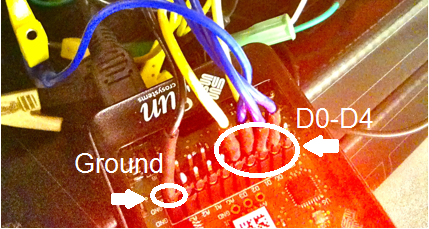
\includegraphics{img/sunspotconnections1.png}
\caption{The Sun SPOT with connections added to the ground and the digital
I/O}
\end{figure}


% }}}

\subsubsection{Bit banging: hardware bus} % {{{

Now that we have both the Cobot ready to drive and the bit-banging between the
Sun SPOTs. We can finally start putting the pieces together. Although we had all
the pieces, it was still hard to get them to work together properly.  The main
problem was touched on in the last part. The difference is voltage the two
pieces of hardware used. The Cobot uses a voltage of 5 and the Sun SPOT a
voltage of 3. This gives problems when you, want to send signals to from the
Cobot to the Sun SPOT.  \begin{equation} \label{eq:voltage} U = I*R
\end{equation}
So to solve this problem we had to make a wire with 2 serial resistances of 300
and 200 K $\Omega$. This makes sure only 3V gets to the Sun Spot and the
other 2V leaks out through the other side to the ground. Like you can see in
figure \ref{fig:handshaking}.
This solution is not valid if you are trying to send more complex information
than just a giving a high signal, because the message will get distorted if
there is a resistance between the sender and receiver.
% Not sure about this explaination

% TODO: figure of the resistance.
Also, we initially used timers for the Sun SPOTs to send datagrams to each
other. We could not use this timers from the Java code, since those timers did
not guarantee that a bit is transmitted: there is no guarantee the timers of
both devices are working correctly. We went for a deterministic approach by
implementing a state machine. The basic idea is really simple (you could only
transition from one state into another), but you have to make sure acknowledge
bits are continuously sent to both sides. In figure ~\ref{fig:handshaking} is
shown how the transmission protocol for bit banging works, without using a
clock.

\begin{figure}[H]
\label{fig:handshaking}
\centering
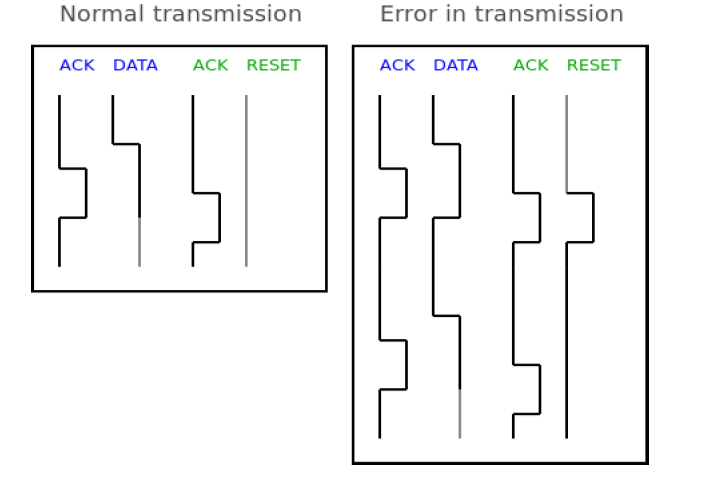
\includegraphics[width=11cm]{img/handshaking.png}
\caption{The left image is a bit diagram of a normal transmission and right is a
simplified example of an error occurred during the transmission. To send one bit
from a device (blue labelled lines; sender) to another device (green labelled
lines; receiver), first put your data pin on the value you want to send. Then
you put your ACK flag on. Now, the receiver knows the sender is ready to send a
bit.  When the receiver sees the sender's ACK flag, the receiver read the value
of the data pin and puts his acknowledge flag on. When the receiver set its ACK
flag, the sender knows the message bit is received. The sender lowers its
acknowledge flag, and the receiver will followed by lowering its own ACK flag as
well. When both ACK flags are down, the process starts all over again. There is
also a reset flag, which indicates a restart of the whole process is required.
The receiver will set its reset flag, when an invalid value is received.}
\end{figure}

% }}}

% }}}

\pagebreak

\section{Implementation} % {{{
\label{sec:Implementation}

\subsection{Cobot implementation} % {{{
\label{sub:Cobot implementation}

Since there was no manual or documentation available about the toolchain, nor
about the internals of the Jobot, the first week's progress of this assignment
was slow. Most of the time, we were trying to solve problems and looking for
more information about the microcontroller and servos on the internet.
Eventually, when all tools for the toolchain were obtained and successfully
working together, we were able to run example code on the Jobot. This was the
breakthrough we were waiting for: we were able to write our own code and program
the Jobot with our compiled source code.

\subsubsection{The first working example source code} % {{{
\label{ssub:The first working example source code}

When we were using the PCH version of the CCS C compiler, we found some example
source code in the directory of the CCS C compiler. We modified the example code
to proof the microcontroller can do something, and programmed this modified code
on the Jobot's microcontroller:

\begin{Verbatim}[commandchars=\\\{\}]
\PY{c+c1}{// Device configuration: 20 Mhz processor and enable rs232,}
\PY{c+c1}{// which is the COM port. The COM port uses a baudrate of 9600.}
\PY{c+cp}{#}\PY{c+cp}{if defined(\PYZus{}\PYZus{}PCH\PYZus{}\PYZus{})}
\PY{c+cp}{#}\PY{c+cp}{include "18f452.h"}
\PY{c+cp}{#}\PY{c+cp}{fuses HS,NOPROTECT}
\PY{c+cp}{#}\PY{c+cp}{use delay(clock=20000000)}
\PY{c+cp}{#}\PY{c+cp}{use rs232(baud=9600, xmit=PIN\PYZus{}C6, rcv=PIN\PYZus{}C7)}
\PY{c+cp}{#}\PY{c+cp}{endif}

\PY{k+kt}{void} \PY{n+nf}{main}\PY{p}{(}\PY{p}{)} \PY{p}{\PYZob{}}
    \PY{c+c1}{// Set B pins to 'output' mode}
    \PY{n}{set\PYZus{}tris\PYZus{}b}\PY{p}{(}\PY{l+m+mi}{0}\PY{p}{)}\PY{p}{;}

    \PY{c+c1}{// Blink two LEDs (located on the microcontroller board).}
    \PY{c+c1}{// Wait for 2 ms between toggling the pins' value.}
    \PY{k}{while}\PY{p}{(}\PY{l+m+mi}{1}\PY{p}{)} \PY{p}{\PYZob{}}
        \PY{n}{output\PYZus{}high}\PY{p}{(}\PY{n}{PIN\PYZus{}B1}\PY{p}{)}\PY{p}{;}
        \PY{n}{delay\PYZus{}us}\PY{p}{(}\PY{l+m+mi}{2000}\PY{p}{)}\PY{p}{;}
        \PY{n}{output\PYZus{}low}\PY{p}{(}\PY{n}{PIN\PYZus{}B1}\PY{p}{)}\PY{p}{;}

        \PY{n}{output\PYZus{}high}\PY{p}{(}\PY{n}{PIN\PYZus{}B3}\PY{p}{)}\PY{p}{;}
        \PY{n}{delay\PYZus{}us}\PY{p}{(}\PY{l+m+mi}{2000}\PY{p}{)}\PY{p}{;}
        \PY{n}{output\PYZus{}low}\PY{p}{(}\PY{n}{PIN\PYZus{}B3}\PY{p}{)}\PY{p}{;}
    \PY{p}{\PYZcb{}}
\PY{p}{\PYZcb{}}
\end{Verbatim}


\noindent Note: The code shown above is a heavily modified version of the
example file \texttt{ex\_led.c}, which is part of the CCS C compiler's examples.

% }}}

\subsubsection{Cobot's data receiver and error checker} % {{{
\label{ssub:Cobot's data receiver and error checker}

\begin{Verbatim}[commandchars=\\\{\}]
\PY{c+c1}{// Buffer for data receiving}
\PY{k+kt}{int} \PY{n}{data\PYZus{}previous}\PY{p}{,} \PY{n}{data\PYZus{}current}\PY{p}{,} \PY{n}{data\PYZus{}received}\PY{p}{,} \PY{n}{receive\PYZus{}round}\PY{p}{;}
\PY{k+kt}{int} \PY{n}{b}\PY{p}{,} \PY{n}{bit\PYZus{}count} \PY{o}{=} \PY{l+m+mi}{3}\PY{p}{;}

\PY{k+kt}{void} \PY{n+nf}{receive\PYZus{}data}\PY{p}{(}\PY{p}{)} \PY{p}{\PYZob{}}
    \PY{c+c1}{// Clear data buffers}
    \PY{n}{data\PYZus{}received} \PY{o}{=} \PY{n}{data\PYZus{}previous} \PY{o}{=} \PY{n}{data\PYZus{}current} \PY{o}{=} \PY{l+m+mi}{0}\PY{p}{;}

    \PY{c+c1}{// Receive two times (= "rounds") three bits. Most significant bits are}
    \PY{c+c1}{// transmitted first (thus from left to right)}
    \PY{k}{for}\PY{p}{(} \PY{n}{receive\PYZus{}round} \PY{o}{=} \PY{l+m+mi}{0}\PY{p}{;} \PY{n}{receive\PYZus{}round} \PY{o}{<} \PY{l+m+mi}{2}\PY{p}{;} \PY{n}{receive\PYZus{}round}\PY{o}{+}\PY{o}{+} \PY{p}{)} \PY{p}{\PYZob{}}
        \PY{k}{for}\PY{p}{(}\PY{n}{b} \PY{o}{=} \PY{l+m+mi}{0}\PY{p}{;} \PY{n}{b} \PY{o}{<} \PY{n}{bit\PYZus{}count}\PY{p}{;} \PY{n}{b}\PY{o}{+}\PY{o}{+}\PY{p}{)} \PY{p}{\PYZob{}}
            \PY{c+c1}{//printf("round: %d, b: %d\PYZbs{}n", receive\PYZus{}round, bit\PYZus{}count - b);}
            \PY{n}{debug}\PY{p}{(}\PY{l+s}{"}\PY{l+s}{get\PYZus{}sender\PYZus{}ack() first}\PY{l+s+se}{\PYZbs{}n}\PY{l+s}{"}\PY{p}{)}\PY{p}{;}
            \PY{k}{while}\PY{p}{(}\PY{o}{!}\PY{n}{get\PYZus{}sender\PYZus{}ack}\PY{p}{(}\PY{p}{)}\PY{p}{)}
                \PY{n}{wait}\PY{p}{(}\PY{l+m+mi}{1}\PY{p}{)}\PY{p}{;}

            \PY{n}{debug}\PY{p}{(}\PY{l+s}{"}\PY{l+s}{get\PYZus{}sender\PYZus{}data()}\PY{l+s+se}{\PYZbs{}n}\PY{l+s}{"}\PY{p}{)}\PY{p}{;}
            \PY{n}{data\PYZus{}current} \PY{o}{|}\PY{o}{=} \PY{n}{get\PYZus{}sender\PYZus{}data}\PY{p}{(}\PY{p}{)} \PY{o}{<}\PY{o}{<} \PY{p}{(}\PY{n}{bit\PYZus{}count}\PY{o}{-}\PY{n}{b}\PY{o}{-}\PY{l+m+mi}{1}\PY{p}{)}\PY{p}{;}

            \PY{c+c1}{// First round is simply storing the data and emits an acknowledge}
            \PY{c+c1}{// signal (= 1). The second round is used for error checking. The}
            \PY{c+c1}{// second round will emit an acknowledge signal when the data is}
            \PY{c+c1}{// properly transmitted / received. The second round will send an}
            \PY{c+c1}{// acknowledge and reset signal (= 3), when the current data bit is}
            \PY{c+c1}{// not matching data of the previous round.}
            \PY{k}{if}\PY{p}{(}\PY{n}{receive\PYZus{}round} \PY{o}{=}\PY{o}{=} \PY{l+m+mi}{0}
                    \PY{o}{|}\PY{o}{|} \PY{p}{(}\PY{n}{data\PYZus{}previous} \PY{o}{&} \PY{p}{(}\PY{l+m+mi}{1}\PY{o}{<}\PY{o}{<}\PY{p}{(}\PY{n}{bit\PYZus{}count}\PY{o}{-}\PY{n}{b}\PY{o}{-}\PY{l+m+mi}{1}\PY{p}{)}\PY{p}{)}\PY{p}{)}
                            \PY{o}{=}\PY{o}{=} \PY{p}{(}\PY{n}{data\PYZus{}current} \PY{o}{&} \PY{p}{(}\PY{l+m+mi}{1}\PY{o}{<}\PY{o}{<}\PY{p}{(}\PY{n}{bit\PYZus{}count}\PY{o}{-}\PY{n}{b}\PY{o}{-}\PY{l+m+mi}{1}\PY{p}{)}\PY{p}{)}\PY{p}{)}\PY{p}{)}
                \PY{n}{set\PYZus{}output}\PY{p}{(}\PY{l+m+mi}{1}\PY{p}{)}\PY{p}{;}
            \PY{k}{else} \PY{p}{\PYZob{}}
                \PY{n}{debug}\PY{p}{(}\PY{l+s}{"}\PY{l+s}{Error during transmission}\PY{l+s+se}{\PYZbs{}n}\PY{l+s}{"}\PY{p}{)}\PY{p}{;}
                \PY{n}{set\PYZus{}output}\PY{p}{(}\PY{l+m+mi}{3}\PY{p}{)}\PY{p}{;}

                \PY{c+c1}{// Wait until the sender sees the acknowledge and reset signal.}
                \PY{c+c1}{// When the sender emits his acknowledge signal, the receive}
                \PY{c+c1}{// procedure is restarted.}
                \PY{k}{while}\PY{p}{(}\PY{n}{get\PYZus{}sender\PYZus{}ack}\PY{p}{(}\PY{p}{)}\PY{p}{)}
                    \PY{n}{wait}\PY{p}{(}\PY{l+m+mi}{1}\PY{p}{)}\PY{p}{;}
                \PY{n}{set\PYZus{}output}\PY{p}{(}\PY{l+m+mi}{0}\PY{p}{)}\PY{p}{;}
                \PY{k}{return} \PY{n}{receive\PYZus{}data}\PY{p}{(}\PY{p}{)}\PY{p}{;}
            \PY{p}{\PYZcb{}}

            \PY{n}{debug}\PY{p}{(}\PY{l+s}{"}\PY{l+s}{get\PYZus{}sender\PYZus{}ack() last}\PY{l+s+se}{\PYZbs{}n}\PY{l+s}{"}\PY{p}{)}\PY{p}{;}
            \PY{k}{while}\PY{p}{(}\PY{n}{get\PYZus{}sender\PYZus{}ack}\PY{p}{(}\PY{p}{)}\PY{p}{)}
                \PY{n}{wait}\PY{p}{(}\PY{l+m+mi}{1}\PY{p}{)}\PY{p}{;}

            \PY{n}{set\PYZus{}output}\PY{p}{(}\PY{l+m+mi}{0}\PY{p}{)}\PY{p}{;}
        \PY{p}{\PYZcb{}}

        \PY{n}{data\PYZus{}previous} \PY{o}{=} \PY{n}{data\PYZus{}current}\PY{p}{;}
        \PY{n}{data\PYZus{}current} \PY{o}{=} \PY{l+m+mi}{0}\PY{p}{;}
    \PY{p}{\PYZcb{}}

    \PY{n}{data\PYZus{}received} \PY{o}{=} \PY{n}{data\PYZus{}previous}\PY{p}{;}
\PY{p}{\PYZcb{}}
\end{Verbatim}


% }}}

% }}}

\subsection{Sun SPOT implementation} % {{{
\label{sub:Sun SPOT implementation}

For this project we used one Sunspot to determine the movement of the robot (by
measuring the tilt) and sending that information using a wireless connection to
the other Sun SPOT. The other Sun SPOT will receive the datagram sent and uses
bit banging to send the received movement to the Cobot. Both Sun SPOTs start up
a \texttt{BootloaderListenerService}, so that we can read the debug output at
real-time on our computer. This was very useful to debug the Java code. Both
Sunspots extend the \texttt{javax.microedition.midlet.MIDlet} class, so that all
the functions the Sun SPOT needs to operate are in the code.

\subsubsection{Measure tilt and send wireless datagrams.} % {{{

Two threads are used to enable measuring tilt while sending datagrams. It is
necessary to create two threads, because sending/receiving datagrams is a
blocking operation. If a single thread is used for both tasks, the tilt is not
measured until the sending/receiving process is done.
\\
\\
\noindent Thread 1: \textbf{Measuring the tilt and determine what the next Cobot's
movement is or if the Cobot should halt.}
\\
\\
This thread continuously measures the tilt of the Sunspot. After measuring the
tilt, the next movement of the Cobot is determined by checking if the Y tilt is
larger than the X direction and by measuring if the tilt of either the Y or the
X direction is larger than 25 degrees. When this is not the case, the Sunspot
will set the movement to ``stop'' (thus no movement). If this is the case and X
is larger than Y, the Sunspot will set the direction to left or right. If the
tilt is negative, the Sun SPOT will turn right and vice versa.  Pretty much the
same case if the tilt in the Y direction is larger than the tilt in the X
direction. After the movement of the Cobot is determined, the LEDs are set in
such way that it is clear what is measured. The code of thread 1:

\begin{Verbatim}[commandchars=\\\{\}]
\PY{k}{new} \PY{n+nf}{Thread}\PY{o}{(}\PY{o}{)} \PY{o}{\PYZob{}}
    \PY{k+kd}{public} \PY{k+kt}{void} \PY{n+nf}{run}\PY{o}{(}\PY{o}{)} \PY{o}{\PYZob{}}
        \PY{k+kt}{int} \PY{n}{tiltX} \PY{o}{=} \PY{l+m+mi}{0}\PY{o}{;}
        \PY{k+kt}{int} \PY{n}{tiltY} \PY{o}{=} \PY{l+m+mi}{0}\PY{o}{;}
        \PY{k}{while} \PY{o}{(}\PY{k+kc}{true}\PY{o}{)} \PY{o}{\PYZob{}}
            \PY{k}{try} \PY{o}{\PYZob{}}
                \PY{c+cm}{/* Measure the degrees. */}
                \PY{n}{tiltX} \PY{o}{=} \PY{o}{(}\PY{k+kt}{int}\PY{o}{)} \PY{n}{Math}\PY{o}{.}\PY{n+na}{toDegrees}\PY{o}{(}\PY{n}{accel}\PY{o}{.}\PY{n+na}{getTiltX}\PY{o}{(}\PY{o}{)}\PY{o}{)}\PY{o}{;}
                \PY{n}{tiltY} \PY{o}{=} \PY{o}{(}\PY{k+kt}{int}\PY{o}{)} \PY{n}{Math}\PY{o}{.}\PY{n+na}{toDegrees}\PY{o}{(}\PY{n}{accel}\PY{o}{.}\PY{n+na}{getTiltY}\PY{o}{(}\PY{o}{)}\PY{o}{)}\PY{o}{;}
                \PY{n}{result} \PY{o}{=} \PY{n}{STOP}\PY{o}{;}

                \PY{c+cm}{/*}
\PY{c+cm}{                 * If the Sunspot is in a bigger sideways tilt than a}
\PY{c+cm}{                 * frontal tilt. If none of the tilts is more than 15,}
\PY{c+cm}{                 * the Sunspot is in a STOP state.}
\PY{c+cm}{                 */}
                \PY{k}{if} \PY{o}{(}\PY{o}{(}\PY{n}{Math}\PY{o}{.}\PY{n+na}{abs}\PY{o}{(}\PY{n}{tiltX}\PY{o}{)} \PY{o}{>} \PY{n}{Math}\PY{o}{.}\PY{n+na}{abs}\PY{o}{(}\PY{n}{tiltY}\PY{o}{)}\PY{o}{)}
                        \PY{o}{&}\PY{o}{&} \PY{n}{Math}\PY{o}{.}\PY{n+na}{abs}\PY{o}{(}\PY{n}{tiltX}\PY{o}{)} \PY{o}{>} \PY{n}{ANGLE}\PY{o}{)} \PY{o}{\PYZob{}}
                    \PY{k}{if} \PY{o}{(}\PY{n}{tiltX} \PY{o}{<} \PY{l+m+mi}{0}\PY{o}{)} \PY{o}{\PYZob{}}
                        \PY{n}{result} \PY{o}{=} \PY{n}{RIGHT}\PY{o}{;}
                    \PY{o}{\PYZcb{}} \PY{k}{else} \PY{o}{\PYZob{}}
                        \PY{n}{result} \PY{o}{=} \PY{n}{LEFT}\PY{o}{;}
                    \PY{o}{\PYZcb{}}
                \PY{o}{\PYZcb{}} \PY{k}{else} \PY{k}{if} \PY{o}{(}\PY{o}{(}\PY{n}{Math}\PY{o}{.}\PY{n+na}{abs}\PY{o}{(}\PY{n}{tiltX}\PY{o}{)} \PY{o}{<} \PY{n}{Math}\PY{o}{.}\PY{n+na}{abs}\PY{o}{(}\PY{n}{tiltY}\PY{o}{)}\PY{o}{)}
                        \PY{o}{&}\PY{o}{&} \PY{n}{Math}\PY{o}{.}\PY{n+na}{abs}\PY{o}{(}\PY{n}{tiltY}\PY{o}{)} \PY{o}{>} \PY{n}{ANGLE}\PY{o}{)} \PY{o}{\PYZob{}}
                    \PY{k}{if} \PY{o}{(}\PY{n}{tiltY} \PY{o}{>} \PY{l+m+mi}{0}\PY{o}{)} \PY{o}{\PYZob{}}
                        \PY{n}{result} \PY{o}{=} \PY{n}{DRIVE}\PY{o}{;}
                    \PY{o}{\PYZcb{}} \PY{k}{else} \PY{o}{\PYZob{}}
                        \PY{n}{result} \PY{o}{=} \PY{n}{REVERSE}\PY{o}{;}
                    \PY{o}{\PYZcb{}}
                \PY{o}{\PYZcb{}}
                \PY{c+cm}{/* Set the result on the leds. */}
                \PY{n}{set\PYZus{}Leds}\PY{o}{(}\PY{n}{result}\PY{o}{)}\PY{o}{;}
            \PY{o}{\PYZcb{}} \PY{k}{catch} \PY{o}{(}\PY{n}{IOException} \PY{n}{ex}\PY{o}{)} \PY{o}{\PYZob{}} \PY{o}{\PYZcb{}}
        \PY{o}{\PYZcb{}}
    \PY{o}{\PYZcb{}}
\PY{o}{\PYZcb{}}\PY{o}{.}\PY{n+na}{start}\PY{o}{(}\PY{o}{)}\PY{o}{;}
\end{Verbatim}


\noindent The constants ANGLE, RIGHT, LEFT, STOP, DRIVE and REVERSE are
specified in the main class. The constant ANGLE is set to \texttt{15} (= minimum
degrees used to filter unintended movements). The constants RIGHT, LEFT, STOP,
DRIVE and REVERSE are movement identifiers, since only bits are transferred
between the Sun SPOTs and the Sun SPOT and the Jobot, it is better to create
readable identifiers.
\\
\\
\noindent Thread 2: \textbf{Sending a wireless package to the other Sunspot
containing the direction.}
\\
\\
This thread determines if the movement variable has been changed. If the
movement variable has changed, it will send a radiogram containing the
corresponding value of the movement to the other sunspot. Before this is
possible, a radio connection has to be established. The connection is made using
this function call: \texttt{Connector.open("radiogram://broadcast:37")}.

And a so called ``datagram'' has to be made. We write the integer that contains
the direction information to the datagram and this datagram is send to the other
Sunspot. The code of thread 2:

\begin{Verbatim}[commandchars=\\\{\}]
\PY{k}{new} \PY{n+nf}{Thread}\PY{o}{(}\PY{o}{)} \PY{o}{\PYZob{}}
    \PY{k+kd}{public} \PY{k+kt}{void} \PY{n+nf}{run}\PY{o}{(}\PY{o}{)} \PY{o}{\PYZob{}}
        \PY{c+cm}{/* We create a DatagramConnection */}
        \PY{n}{DatagramConnection} \PY{n}{dgConnection} \PY{o}{=} \PY{k+kc}{null}\PY{o}{;}
        \PY{n}{Datagram} \PY{n}{dg} \PY{o}{=} \PY{k+kc}{null}\PY{o}{;}
        \PY{k}{try} \PY{o}{\PYZob{}}
            \PY{n}{dgConnection} \PY{o}{=}
                \PY{o}{(}\PY{n}{DatagramConnection}\PY{o}{)} \PY{n}{Connecor}\PY{o}{.}\PY{n+na}{open}\PY{o}{(}\PY{l+s}{"radiogram://broadcast:37"}\PY{o}{)}\PY{o}{;}
            \PY{c+cm}{/* Ask for a datagram with the maximum size allowed */}
            \PY{n}{dg} \PY{o}{=} \PY{n}{dgConnection}\PY{o}{.}\PY{n+na}{newDatagram}\PY{o}{(}\PY{n}{dgConnection}\PY{o}{.}\PY{n+na}{getMaximumLength}\PY{o}{(}\PY{o}{)}\PY{o}{)}\PY{o}{;}
        \PY{o}{\PYZcb{}} \PY{k}{catch} \PY{o}{(}\PY{n}{IOException} \PY{n}{ex}\PY{o}{)} \PY{o}{\PYZob{}}
            \PY{n}{System}\PY{o}{.}\PY{n+na}{out}\PY{o}{.}\PY{n+na}{println}\PY{o}{(}\PY{l+s}{"Could not open radiogram connection"}\PY{o}{)}\PY{o}{;}
            \PY{k}{return}\PY{o}{;}
        \PY{o}{\PYZcb{}}

        \PY{k}{while} \PY{o}{(}\PY{k+kc}{true}\PY{o}{)} \PY{o}{\PYZob{}}
            \PY{k}{try} \PY{o}{\PYZob{}}
                \PY{c+cm}{/*}
\PY{c+cm}{                 * If there is a change in direction, send the direction}
\PY{c+cm}{                 * in the form of an integer to an other Sunspot.}
\PY{c+cm}{                 */}
                \PY{k}{if} \PY{o}{(}\PY{n}{result} \PY{o}{!}\PY{o}{=} \PY{n}{result\PYZus{}old}\PY{o}{)} \PY{o}{\PYZob{}}
                    \PY{n}{result\PYZus{}old} \PY{o}{=} \PY{n}{result}\PY{o}{;}
                    \PY{n}{dg}\PY{o}{.}\PY{n+na}{reset}\PY{o}{(}\PY{o}{)}\PY{o}{;}
                    \PY{n}{dg}\PY{o}{.}\PY{n+na}{writeInt}\PY{o}{(}\PY{n}{result}\PY{o}{)}\PY{o}{;}
                    \PY{n}{dgConnection}\PY{o}{.}\PY{n+na}{send}\PY{o}{(}\PY{n}{dg}\PY{o}{)}\PY{o}{;}
                    \PY{n}{System}\PY{o}{.}\PY{n+na}{out}\PY{o}{.}\PY{n+na}{println}\PY{o}{(}\PY{l+s}{"Broadcast is going through"}\PY{o}{)}\PY{o}{;}
                \PY{o}{\PYZcb{}}
            \PY{o}{\PYZcb{}} \PY{k}{catch} \PY{o}{(}\PY{n}{IOException} \PY{n}{ex}\PY{o}{)} \PY{o}{\PYZob{}} \PY{o}{\PYZcb{}}
        \PY{o}{\PYZcb{}}
    \PY{o}{\PYZcb{}}
\PY{o}{\PYZcb{}}\PY{o}{.}\PY{n+na}{start}\PY{o}{(}\PY{o}{)}\PY{o}{;}
\end{Verbatim}


% }}}

\subsubsection{Receive movement and communicate with Cobot} % {{{
TODO ...
\\
\\
\noindent Thread 1: \textbf{Receive the datagrams sent by the Sun SPOT.}
\\
\\
After the direction has been sent, the Sun SPOT sets the LEDs in a way that
it is clear what the received direction is. It will also start up the bit
banging process.

% }}}

\subsubsection{Sun SPOT / Cobot handshake} % {{{
\label{ssub:Sun SPOT / Cobot handshake}

Before the second Sun SPOT starts receiving, it first needs to get a handshake
from the Cobot. The handshake is given when the Sunspot receives two high
signals on the digital pins that are used for input. If the Sunspot receives a
high signal on the reset input pin after the handshake, the Cobot didn't receive
the bits like they were send. When this happens, the same byte is send again
(twice for checking) to the Cobot. Every step of the bit banging process has to
get conformation from the Cobot that everything is OK. This is done by setting
the pins in a certain way. For more information about how the initial handshake
is done, we refer to the comments in the Sun SPOT and Cobot source code.

% }}}

%\subsubsection{Tilt control and use} % {{{
% TODO: describe protocol for turning tilt information into control functions,
% and then describe how the user interacts with the system and the LEDs help
% with this.




%Thread 1: Receive the datagrams sent by the Sun SPOT.

%After the direction has been sent, the Sun SPOT sets the LEDs in a way that
%it is clear what the received direction is. It will also start up the bit
%banging process.

% }}}

% }}}

% }}}

%\section{Results} % {{{
%\label{sec:Results}
%%Not the same as the Conclusion in this case?
%% }}}

%Not the same as the Conclusion in this case? -- no:
% TODO: results should describe the behaviour of the cobot implementation,
%including serial output; the behaviour of the communications link
%implementation between cobot and sun spot; the behaviour of the Sun SPOT tilt
%implementation; and the overall behaviour of the RC setup.

% }}}

\section{Discussion} % {{{
%think this belongs in the discussion cause this you talk about the problems
% you had while doing the project.
% TODO: might want to add what ever is on your heart.
While we were doing the project there were a lot of hurdles to overcome which
were not necessarily part of the project. Some of the materials were lacking
or not available at the time :like there were not enough working batteries.
The software used for the project was not available on the computers(Sun SPOT
manager, ANT and the SDK). Also,
the robots mainly use a com port to do the programming which mostly not
available anymore on most of the newer computers and laptops. but I think
the efforts we made this year will make it proceed more smoothly in the coming
years. This project taught us more than just how to work with program robots
but also the hardships you have to deal with if were to start your own project.
In the end thinking out of the box and hard work paid off. Because we
got the robot working in the end.
% }}}

\section{Results and conclusion} % {{{
% TODO: explain characteristics of the behaviour, and any differences between
% the behaviour and the expected behaviour.

% TODO: What we've learned, what we might have done better, what we did well.

% Have moved the future bit into the conclusion:
With all the code we have right now the most logical step would be to use Cobots
and let them communicate. One Cobot would be the master and the other one the
slave. We would give the master a route to walk and we would want the slave to
follow the master. After this we could use the sensors on the Cobot to avoid
collision and let it autonomously wander. While still sending information to the
slave to follow it. The list goes on and on. There were so many other things we
wanted to do, but cause of lack of time we could not.


% }}}

\section{Acknowledgements} % {{{

% TODO: teaching staff (names) for technical building potential divider, adapted
% pins and wires, and for attaching the Cobot's prorgramming port connector.
% James Caska and Peter van Lith for providing tips, manuals and diagrams for
% programming the Jobot without the Muvium Java layer.

% }}}

\pagebreak

\appendix

\section{Robot hardware specification} % {{{
\label{app:robot-hardware}

This section describes the hardware characteristics of key tools and devices
used in this project.

\subsection{Sun SPOT} % {{{
\label{app:Sun SPOT}

The Sun SPOT Device is a small, wireless, battery powered experimental platform.
It is programmed almost entirely in Java (hence the name ``Sun'', main developer
of the Java platform, in ``Sun SPOT'') to allow regular programmers to create
projects that used to require specialized embedded system development skills.
The hardware platform includes a range of built-in sensors as well as the
ability to easily interface to external devices.

Each Sun SPOT has a 180MHz 32-bit ARM920T core processor with 512Kb RAM and 4Mb
Flash. The sensor board contains:

\begin{itemize}
    \item One 3-axis accelerometer (with two range settings: 2G or 6G).
    \item One temperature sensor.
    \item One light sensor.
    \item Eight tri-color LEDs.
    \item Six analog inputs readable by an ADC.
    \item Two momentary switches.
    \item Five general purpose I/O pins.
    \item Four high current output pins.
    \item $2.4 GHz$ IEEE $802.15.4$ radio with integrated antenna;
    \item $AT91$ timer chip;
    \item USB interface;
    \item $2G/6G$ three-axis accelerometer;
    \item One temperature sensor;
    \item One light sensor;
    % \item 8 tri-color LEDs;
    % \item 6 analog inputs;
    % \item 2 momentary switches;
    % \item 5 general purpose I/O pins;
    % \item 4 high current output pins;
    \item $3.7V$ rechargeable $750 mAh$ lithium-ion battery;
\end{itemize}

We also have a radio sensor board. The Sun SPOTs use a fully capable Java ME
implementation, called Squawk, that supports CLDC 1.1 and MIDP 1.0, plus
provides basic OS functionality. The VM executes directly out of flash memory.
All the device drivers are also written in Java, only a minimal part of the
virtual machine is written in C.

% }}}

\subsection{Jobot/Cobot} % {{{
\label{app:cobot}

\begin{itemize}
    \item PIC16F452 microcontroller with max $40MHz$ CPU clock, 256 byte
    EEPROM data, $32KB$ program memory
    \item Digital communication peripherals (1-A/E/USART, 1-MSSP(SPI/I2C))
    \item Three servos
    \item Three IR sensors
\end{itemize}

% }}}

\subsection{Hemisson} % {{{
\label{sub:Hemisson}

The Hemisson is a two-wheeled robot designed for mobility, that includes:
\begin{itemize}
    \item a PIC16F877 microcontroller with $20MHz$ CPU clock, 8bit,
    $8K$ $\times$ 14 bit words program memory, 368 bytes data memory, 256 bytes
    EEPROM data memory, 14 interrupts, I/O ports A,B,C,D,E, three timers,
    serial communications (MSSP, USART), parallel communications (PSP), 8
    input channel, 10 bit analog to digital module;
    \item two DC motors for independent control of two wheel. Open loop
    control without encoders;
    \item eight IR ambient light sensors;
    \item six IR obstacle detection sensors;
    \item two line detection sensors;
    \item a standard $9V$ (PP3) battery connector;
    \item serial port with DB9 connector;
    \item a TV remote receiver;
    \item a buzzer;
    \item four LEDs;
    \item four programmable switches;
    \item an extension bus for extra modules;
\end{itemize}

% }}}

\subsection{Tools} % {{{

% TODO: the following tools should include make, and key characteristics.

\subsubsection{Hardware} % {{{

% }}}

\subsubsection{Software} % {{{

% }}}

% }}}

% }}}

\bibliographystyle{plain}
\bibliography{cited}

\end{document}
% vim: foldmethod=marker:
